%%%%%%%%%%%%%%%%%%%%%%%%%%%%%%%%%%%%%%%%%
%  Telemac Documentation
%  Example of the TelemacDoc class
%
%%%%%%%%%%%%%%%%%%%%%%%%%%%%%%%%%%%%%%%%%

%----------------------------------------------------------------------------------------
%	PACKAGES AND OTHER DOCUMENT CONFIGURATIONS
%----------------------------------------------------------------------------------------
\documentclass[Misc]{../../data/TelemacDoc} % Default font size and left-justified equations
%\documentclass[Telemac2D,french]{TelemacDoc} % Default font size and left-justified equations in french

\begin{document}

\let\cleardoublepage\clearpage

%----------------------------------------------------------------------------------------
%	TITLE PAGE
%----------------------------------------------------------------------------------------
\title{\telemacsystem}
\subtitle{Developer Guide}
\version{7.2}
\author{Yoann Audouin}
\date{\today}
\maketitle
\clearpage


%----------------------------------------------------------------------------------------
%	COPYRIGHT PAGE
%----------------------------------------------------------------------------------------

\newpage

\thispagestyle{empty}

\TelemacCopyright{}


%----------------------------------------------------------------------------------------
%	TABLE OF CONTENTS
%----------------------------------------------------------------------------------------


\pagestyle{empty} % No headers

\tableofcontents% Print the table of contents itself

%\cleardoublepage % Forces the first chapter to start on an odd page so it's on the right

\pagestyle{fancy} % Print headers again

%----------------------------------------------------------------------------------------
%     Intro
%----------------------------------------------------------------------------------------
%==================================
%==================================
\chapter{Introduction}
%==================================
%==================================
%==================================
\section{A word of caution}
%==================================
This document contains information about the quality of a complex modelling tool. Its purpose is to assist the user in assessing the reliability and accuracy of computational results, and to provide guidelines with respect to the applicability and judicious employment of this tool. This document does not, however, provide mathematical proof of the correctness of results for a specific application. The reader is referred to the License Agreement for pertinent legal terms and conditions associated with the use of the software.

The contents of this validation document attest to the fact that computational modelling of complex physical systems requires great care and inherently involves a number of uncertain factors. In order to obtain useful and accurate results for a particular application, the use of high-quality modelling tools is necessary but not sufficient. Ultimately, the quality of the computational results that can be achieved will depend upon the adequacy of available data as well as a suitable choice of model and modelling parameters.
% 
%==================================
\section{Validation layout}
% %==================================

This validation is presented hereafter using a \textit{validation sheet form},
each sheet detailing the physical concepts involved, the physical and numerical parameters used and comparing both numerical and reference solutions.
Then, each sheet displays the following informations:
\begin{list}{-}{}
\item [-] \textbf{Purpose \& Problem description} : These first two parts give reader short details about the test case, the physical phenomena involved and specify how the numerical solution will be validated;
\item [-] \textbf{Reference} : This part gives the reference solution we are comparing to and explicits the analytical solution when available;
\item [-] \textbf{Physical parameters} : This part specifies the geometry,
details all the physical parameters used to describe both porous media (soil model in particularly) and
solute characteristics (dispersion/diffusion coefficients, soil $\equiv$ pollutant interactions...);
\item [-] \textbf{Geometry and Mesh} : This part describes the mesh used in the \tomawac computation;
\item [-] \textbf{Initial and boundary conditions} : this part details both initial and boundary conditions used to simulate the case ;
\item [-] \textbf{Numerical parameters} : this part is used to specify the numerical parameters used
(adaptive time step, mass-lumping when necessary...);
\item [-] \textbf{Results} : we comment in this part the numerical results against the reference ones,
giving understanding keys and making assumptions when necessary.
\end{list}
%
\bigskip
%
\clearpage
%==================================
%==================================
\chapter{Presentation}
%==================================
%==================================
\section{General}
%==================================
\tomawac is a scientific software which models the changes, both in the time and in the spatial domain, of the power spectrum of wind-driven waves and wave agitation for applications in the oceanic domain, in the intracontinental seas as well as in the coastal zone. The model uses the finite elements formalism for discretizing the sea domain; it is based on the computational subroutines of the TELEMAC system as developed by the EDF R\&D’s Laboratoire National d'Hydraulique et Environnement (LNHE). \tomawac is one of the models making up the TELEMAC system 
The acronym \tomawac being adopted for naming the software was derived from the following English denomination:

TELEMAC-based Operational Model Addressing Wave Action Computation

\tomawac can be used for three types of applications:
\begin{itemize}
\item	Wave climate forecasting a few days ahead, from wind field forecasts. This real time type of application is rather directed to weather-forecasting institutes such as Météo-France, whose one mission consists in predicting continuously the weather developments and, as the case may be, publishing storm warnings.
\item	Hindcasting of exceptional events having severely damaged maritime structures and for which field records are either incomplete or unavailable.
\item	Study of wave climatology and maritime or coastal site features, through the application of various, medium or extreme, weather conditions in order to obtain the conditions necessary to carry out projects and studies (harbour constructions, morphodynamic coastal evolutions, ...).
\end{itemize}

%==================================
\section{Capabilities}
%==================================
 \subsection{Application domain of the model \tomawac}
\label{par31}
\tomawac is designed to be applied from the ocean domain up to the coastal zone. The limits of the application range can be determined by the value of the relative depth d/L, wherein d denotes the water height (in metres) and L denotes the wave length (in metres) corresponding to the peak spectral frequency for irregular waves.

The application domain of \tomawac includes:
\begin{itemize}
\item {\bf the oceanic domain}, characterized by large water depths, i.e. by relative water depths of over 0.5. The dominant physical processes are: wind driven waves, whitecapping dissipation and non-linear quadruplet interactions.
\item {\bf the continental seas and the medium depths}, characterized by a relative water depth ranging from 0.05 to 0.5. In addition to the above processes, the bottom friction, the shoaling (wave growth due to a bottom rise) and the effects of refraction due to the bathymetry and/or to the currents are to be taken into account.
\item {\bf The coastal domain}, including shoals or near-shore areas (relative water depth lower than 0.05). For these shallow water areas, such physical processes as bottom friction, bathymetric breaking, non-linear triad interactions between waves should be included. Furthermore, it could be useful to take into account the effects related to unsteady sea level and currents due to the tide and/or to the weather-dependent surges.
\end{itemize}

Through a so-called finite element spatial discretization, one computational grid may include mesh cells among which the ratio of the largest sizes to the smallest ones may reach or even exceed 100. That is why \tomawac can be applied to a sea domain that is featured by highly variable relative water depths; in particular, the coastal areas can be finely represented.

The application domain of \tomawac does not include the harbour areas and, more generally, all those cases in which the effects of reflection on structures and/or diffraction may not be ignored.

A first version of a diffraction model is available in \tomawac and is able to represent some diffraction effects. The model presents still some limits. It is highly recommended to use phase-resolving models when a detailed simulation of diffraction effects is required (e.g. harbor agitation).

\subsection{Wave interactions with other physical factors}
Several factors are involved in the wave physics and interact to various extents with the waves changing their characteristics. The following main factors should be mentioned:
\begin{itemize}
\item bathymetry and sea bottom geometry (bottom friction, refraction, surf-breaking, non-linear effects of interactions with the bottom, sand rippling...)
\item atmospheric circulation (wind and pressure effects)
\item tide pattern (variation of currents and water heights),
\item three-dimensional oceanic circulation currents,
\item over/underelevations caused by exceptional weather events, resulting in sea levels variations up to several meters (storm, surges).
\end{itemize}
The fine modelling of the interactions between these various physical factors and the waves is generally rather complex and several research projects are currently focused on it. Within the application domain as defined in the previous paragraph, \tomawac models the following interactions:
\begin{itemize}

\item {\bf wave-bathymetry interaction}: the submarine relief data input into \tomawac are constant in time, but the sea level can change in time. In addition to the effects of the sea level variations in time, \tomawac allows to take into account refraction, shoaling, bottom friction and bathymetric breaking. \tomawac simulations can take into account some diffraction effects.
\item {\bf wave-atmosphere interaction}: this interaction is the driving phenomenon in the wave generation, takes part in energy dissipation processes (whitecapping, wave propagation against the wind…) and is involved in the energy transfer. To represent the unsteady behaviour of this interaction, \tomawac requires 10 m wind fields (specification of the couple of horizontal velocity components) with a time step matched to the weather conditions being modelled. These wind fields can be provided either by a meteorological model or from satellite measurements.
\item {\bf wave-current interaction}: the sea currents (as generated either by the tide or by oceanic circulations) may significantly affect the waves according to their intensity. They modify the refractive wave propagation direction, they reduce or increase the wave height according to their propagation direction in relation to the waves and may influence the wave periods if exhibiting a marked unsteady behaviour. In \tomawac, the current field is provided by the couple of horizontal components of its average (or depth-integrated) velocity at the nodes of the computational grid. \tomawac allows to model the frequency changes caused either by the Doppler effect or by the unsteady currents, as well as by an heterogeneous current field.
\end{itemize}
\subsection{ The physical processes modelled in \tomawac}
Those interactions being taken into account by \tomawac have been reviewed and a number of physical events or processes have been mentioned in the previous paragraph. These processes modify the total wave energy as well as the directional spectrum distribution of that energy (i.e. the shape of the directional spectrum of energy). So far, the numerical modelling of these various processes, although some of them are now very well known, is not yet mature and keep on providing many investigation subjects. Considering the brief review of physical interactions given in the previous paragraph, the following physical processes are taken into account and digitally modelled in \tomawac:

{\bf—> Energy source/dissipation processes:}
\begin{itemize}
\item wind driven interactions with atmosphere. Those interactions imply the modelling of the wind energy input into the waves. It is the prevailing source term for the wave energy directional spectrum. The way that spectrum evolves primarily depends on wind velocity, direction, time of action and fetch (distance over which the wind is active). It must be pointed out that the energy which is dissipated when the wind attenuates the waves is not taken into account in \tomawac.
\item 	whitecapping dissipation or wave breaking, due to an excessive wave steepness during wave generation and propagation.
\item 	bottom friction-induced dissipation, mainly occurring in shallow water (bottom grain size distribution, ripples, percolation...)
\item 	dissipation through bathymetric breaking. As the waves come near the coast, they swell due to shoaling until they break when they become to steep.
\item dissipation through wave blocking due to strong opposing currents.
\end{itemize}
{\bf—> Non-linear energy transfer conservative processes:}
\begin{itemize}
\item 	non-linear resonant quadruplet interactions, which is the exchange process prevailing at great depths.
\item 		non-linear triad interactions, which become the prevailing process at small depths.
\end{itemize}
{\bf—> Wave propagation-related processes:}
\begin{itemize}
\item 	 wave propagation due to the wave group velocity and, in case, to the velocity of the medium in which it propagates (sea currents).
\item 	depth-induced refraction which, at small depths, modifies the directions of the wave-ray and then implies an energy transfer over the propagation directions.
\item 	shoaling: wave height variation process as the water depth decreases, due to the reduced wavelength and variation of energy propagation velocity.
\item 	current-induced refraction which also causes a deviation of the wave-ray and an energy transfer over the propagation directions.
\item 	interactions with unsteady currents, inducing frequency transfers (e.g. as regards tidal seas).
\item 	diffraction by a coastal structure (breakwater, pier, etc…) or a shoal, resulting in an energy transfer towards the shadow areas beyond the obstacles blocking the wave propagation. The current version of the diffraction model implemented in \tomawac is able to represent qualitatively some diffraction effects.
\end{itemize}

It should be remembered that, due to the hypothesis adopted in paragraph \ref{par31} about the \tomawac application domain, the reflection (partial or total) from a structure or a pronounced depth irregularity is not addressed by the model.

% %==================================
\chapter{Validation}
% %==================================
%
%==================================
\section{Evolution compared to the previous release}
%==================================
Beside some bugs corrected from the previous version, we can denote two main new phenomenas that are now modelled. 
\begin{itemize}
\item {\bf Strong dissipation through wave blocking due to strong opposing currents.} When water waves meet a strong adverse current, with a velocity that approaches the wave group velocity, waves are blocked. Two options can be now considered in \tomawac to take into account wave blocking effects. The first one considers an equilibrium range spectrum (in the presence of ambient flow) applied as an upper limit for the spectrum  \cite{Hedges1985}. The second one add a dissipative term on the right-hand side of the action balance equation \cite{Westhuys2012}. This leads to one test case {\it called opposing\_current} that tests the two options.  
\item {\bf Dissipation due to vegetation.} When the ratio between vegetation height and water depth is important, vegetation can imply some dissipation. Some methods exist  to modelize this dissipation. The method we chose is based on the formulation proposed by Suzuki et al. \cite{Suzuki2011}. This functionnality leads to 2 new test cases called {\it dean } and {\it veget}. The first one is a realistic simulation with a Fortran user file, the second one is less realistic but without any Fortran user file. 
\end {itemize} 
%==================================
\section{Difference with the previous validation}
%==================================
In this validations we have extended in some cases the number of options for a given tested functionnality. For example, in deferl\_bj78, we do not only test Battle and janssen but two other models are tested. In fetch\_limited, 3 others configurations are tested. Another test case has been added named Triplets, to test dissipation due to triplet interactions according to two different models.

Another difference is the use of automatic graphics that are added to this documentation. Though we kepted the old graphics that were comparing to some experimental data. 
%==================================
%\section{Potentialities tested}
%==================================


%==================================
%\section{Architectures}
%==================================

%==================================
%\section{Test case report}
%==================================


%----------------------------------------------------------------------------------------
%     CUE
%----------------------------------------------------------------------------------------
%
%%%%%%%%%%%%%%%%%%%%%%%%%%%%%%%%%%%%%%%%%%%%%%%%%%%%%%%%%%%%%%%%%%%%%%%%
\chapter{CUE}
%%%%%%%%%%%%%%%%%%%%%%%%%%%%%%%%%%%%%%%%%%%%%%%%%%%%%%%%%%%%%%%%%%%%%%%%
%
The CUE is the bug/development tracker of \telemacsystem.
It is available at the following address \url{cue.opentelemac.org}.
In order to login use your SVN login and password.
%
%
\section{Projects}
%
%
\label{proj}
It is divided in multiple projects:
\begin{itemize}
\item Modules: Those are the modules in the \telemacsystem code.
\item Sites: This concern all the development tools (CUE, CIS, Website...).
\item Supporting scripts: This concerns all the environment scripts (Python and
Perl) as well as parallelism, the automatic installer and the Inputs and
Outputs.
\end{itemize}
\begin{figure}[H]
    \centering
    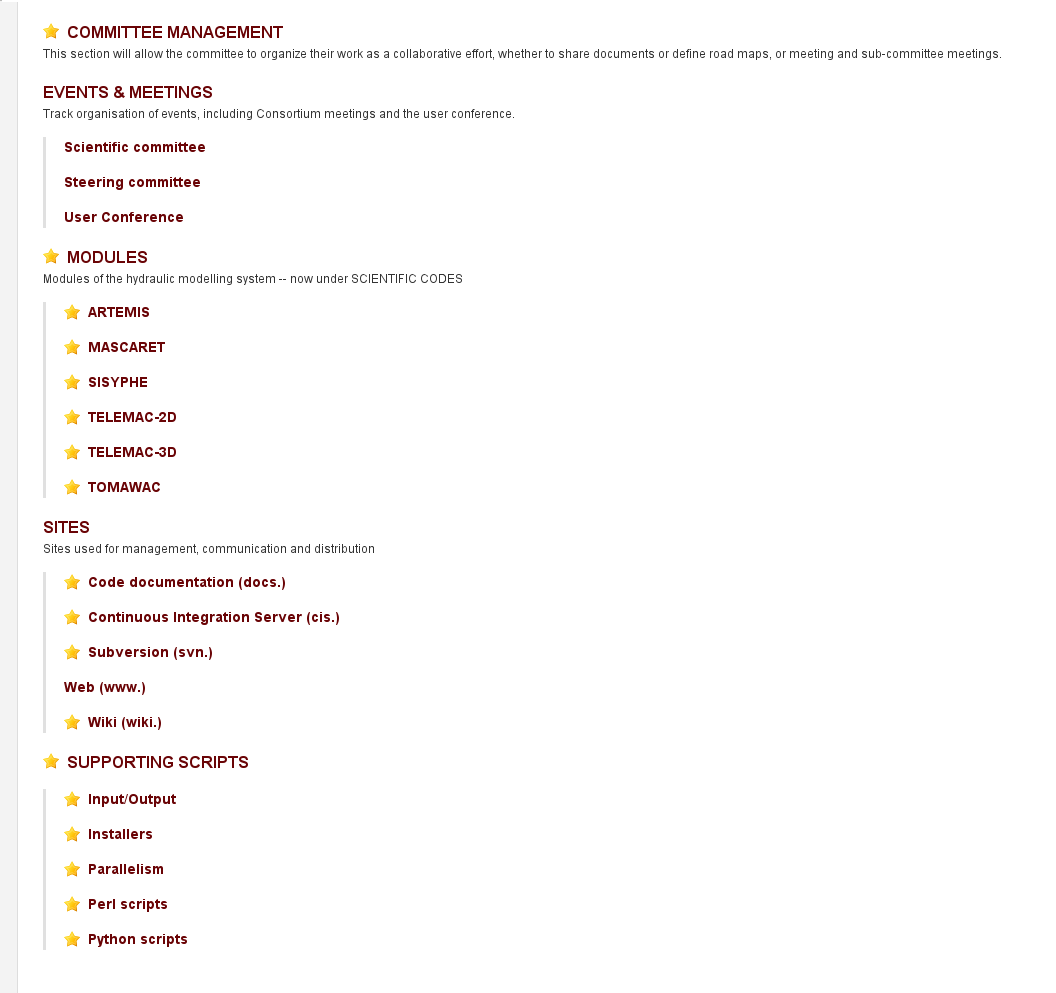
\includegraphics[scale=0.35]{graphics/cue-projects.png}
    \caption{CUE projects}
    \label{fig:cue-projects}
\end{figure}
%
%
\section{Create a ticket}
%
%
To add a new ticket you must go into the project your ticket concern and add
click on "New issue". This will lead you to the page shown on Fig
\ref{fig:cue-ticket}.  You will then need to fill the following information:
\begin{itemize}
\item Tracker: type of the ticket (Bug, Feature, Documentation,
Validation/Verif/Application).
\item Subject: Title of the ticket.
\item Description: Give an full explication of the problem.
\item Status: Status of the ticket (Set to new on creation).
\item Priority: Urgency of the ticket.
\item Assignee: Person in charge of the development integration.
\item Category: Category of the work.
\item Target Version: Version of the code in which the development should be
integrated.
\item Watchers: People that will get an update every time the ticket is
modified.
\end{itemize}
\begin{figure}[H]
    \centering
    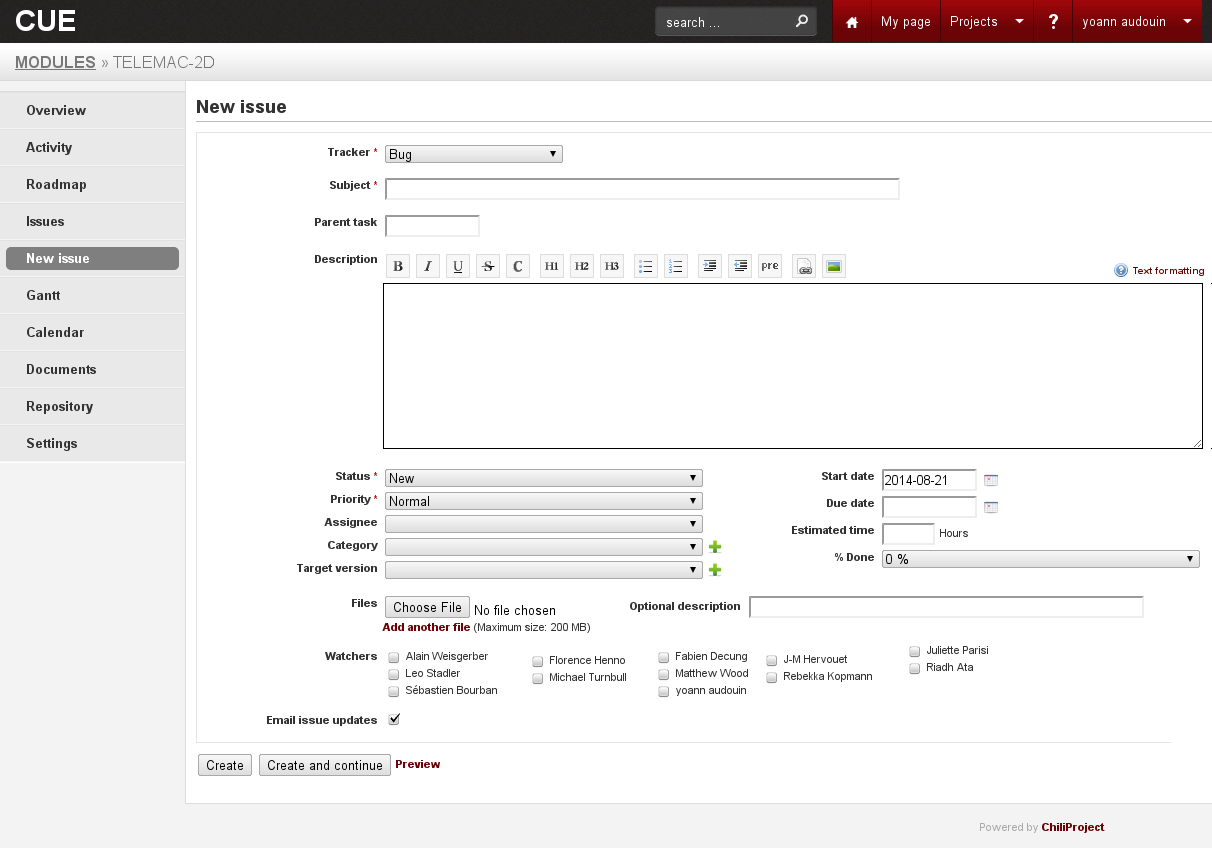
\includegraphics[scale=0.35]{graphics/cue-ticket.png}
    \caption{Creation of a ticket}
    \label{fig:cue-ticket}
\end{figure}

\begin{WarningBlock}{Warning:}
If you do not see the "New issue" button then you forgot to ask in the email
(described in Section \ref{mail}) the project you are working on, you will need
to send a new one to be see that button.
\end{WarningBlock}
%
%
\section{Modify a ticket}
%
%
To Modify a ticket go into the project your ticket is in then click on the
ticket and on the ticket page click on the "update" button in the upper right
corner of the page. The Fig \ref{fig:cue-modify} shows the page you get when
clicking on a ticket.

You will have to update your ticket as your work advance, either by adding
comments on what you have done or by changing its status. For example a bug is
set to "resolved" once we found its solution and set to "closed" once the
correction is integrated in the main version.
%
\begin{figure}[H]
    \centering
    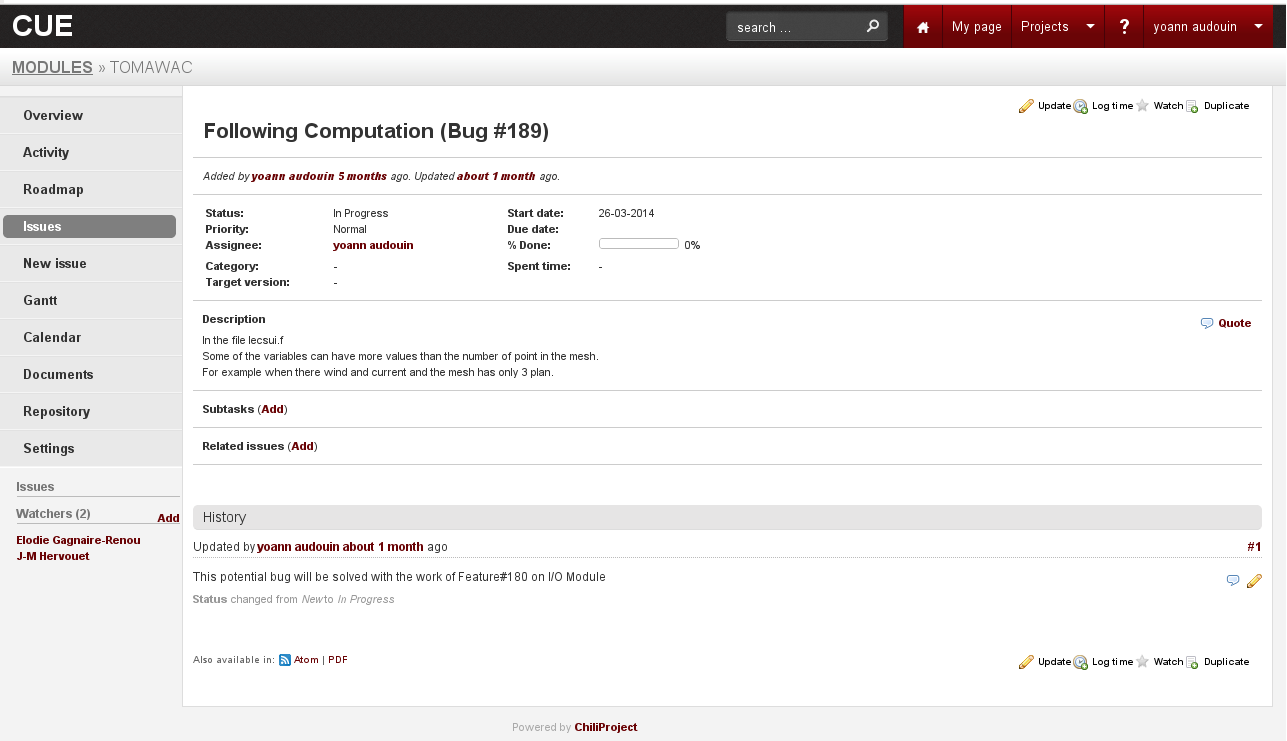
\includegraphics[scale=0.35]{graphics/cue-modify.png}
    \caption{Modification of a ticket}
    \label{fig:cue-modify}
\end{figure}

%
%----------------------------------------------------------------------------------------
%     SVN
%----------------------------------------------------------------------------------------
%----------------------------------------------------------------------------------------------------
\chapter{SVN}
%----------------------------------------------------------------------------------------------------
%
SVN is the name of the software we use to control the source of \telemacsystem. The
link \url{http://en.wikipedia.org/wiki/Version_control} will give you an
explanation of what a source control is.
The section below will give you a guide on how to perform a few actions
using SVN.
%
\begin{figure}[H]
    \centering
    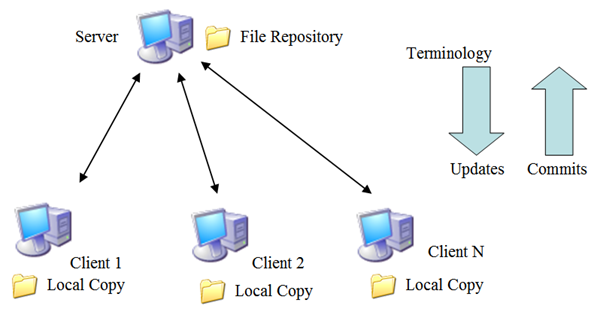
\includegraphics[scale=0.6]{graphics/svn-image.png}
    \caption{SVN structure}
    \label{fig:svn-struct}
\end{figure}
If you are not into command line a few software give you a graphical interface
to handle your repository: kdeSVN, RapidSVN...
%
%
%----------------------------------------------------------------------------------------------------
\section{Create a work copy}
%----------------------------------------------------------------------------------------------------
%
%
\begin{lstlisting}[language=bash]
svn checkout http://svn.opentelemac.org/svn/opentelemac/trunk DEST
\end{lstlisting}
Create a local repository in $DEST$ of the subversion server on the computer.
If you want a working copy of your branch just replace
\url{http://svn.opentelemac.org/svn/opentelemac/trunk} by
\url{http://svn.opentelemac.org/svn/opentelemac/branches/branchname} where
$branchname$ is the name of your branch.\\
%
\begin{WarningBlock}{Warning:}
If your are using a network proxy you need to modify the \verb"$HOME/.subversion/server"
file by adding the following lines under the line \verb"[global]":
\begin{lstlisting}[language=bash]
[global]
...
http-proxy-host = proxypac.edf.fr
http-proxy-port = 3128
http-proxy-username = NNI
http-proxy-password = SesamePassword
...
\end{lstlisting}
Where:
\begin{itemize}
\item \textbf{http-proxy-host} is the address of your proxy.
\item \textbf{http-proxy-port} is the port of your proxy.
\item \textbf{http-proxy-username} is the login for your proxy.
\item \textbf{http-proxy-password} is the password for your proxy.
\end{itemize}
\end{WarningBlock}
%
%
%----------------------------------------------------------------------------------------------------
\section{SVN commands}
%----------------------------------------------------------------------------------------------------
%
%
Here is a list of a few useful SVN commands:
%
\begin{lstlisting}[language=bash]
svn help [command]
\end{lstlisting}
You can get a detailed description of any command.
%
%
\begin{lstlisting}[language=bash]
svn update
\end{lstlisting}
Update your local repository with the server repository. This will add all the
modification made on the subversion server on your local repository.
%
\begin{lstlisting}[language=bash]
svn commit -m "Message about what the commit contains"
\end{lstlisting}
Push your local modifications on the server repository. This will add all the
modifications you made on your local repository on the server repository. You
should alway do an update before doing a commit in case someone else did some
modifications before you. Anyway if you are not up to date SVN will not allow
the commit. The $-m$ option allows you to write directly the message associated
with the commit instead of having a text editor opening. Those messages should
summarize what the commit is adding.\\
The message should respect the following template "[\textit{Type}]
\textit{Text}" where:
\begin{itemize}
\item If you have a cue ticket associated to the commit:
\begin{itemize}
\item Type = "fix \#\textit{id}" ,"feature \#id" or "vnv \#id" where id is the id of
the cue ticket
\item Text = Title of the cue ticket
\end{itemize}
\item Otherwise:
\begin{itemize}
\item Type = doc : If ti concerns the documentation
\item Type = scripts : If it concerns the scripts of the system
\item Type = src : General action on the source code (code convention, trimming removing white spaces...)
\item Type = vnv : Verification \& Validation
\item Text = Description of the commit
\end{itemize}
\end{itemize}
If the commit contains more than one action repeat the process on a new line.
%
\begin{lstlisting}[language=bash]
svn log
\end{lstlisting}
Display all the commit messages.
\\
\begin{CommentBlock}{Tips:}
If the output is too big use the following command instead and press q to exit.
\begin{lstlisting}[language=bash]
svn log|less
\end{lstlisting}
\end{CommentBlock}
%
\begin{lstlisting}[language=bash]
svn status
\end{lstlisting}
Display the status on all the file in the local repository. If a file is
modified, added, missing or deleted. See "svn help status" for more
information.
%
\begin{lstlisting}[language=bash]
svn add/delete/move
\end{lstlisting}
Add/Delete/Move a folder/file to the SVN repository.
%
\begin{lstlisting}[language=bash]
svn info
\end{lstlisting}
Display information about the local repository. Like the address of the server
repository, the last revision, \ldots
%
\begin{lstlisting}[language=bash]
svn revert FILE
\end{lstlisting}
Cancel the local modifications on the file $FILE$. This cannot be undone so
tread lightly with this command.
%
%----------------------------------------------------------------------------------------------------
\section{Update your branch with the latest version of the trunk}
%----------------------------------------------------------------------------------------------------
%
One of the conditions for validating a development is that it is up to date
with the trunk.  In order to ease that step that can be some times painful it
is recommended to do that action weekly.  This way you do smaller updates
instead of a massive one.
\paragraph{The commands}
\begin{enumerate}
\item Go into the branch main folder.
\begin{lstlisting}[language=bash]
cd mybranch
\end{lstlisting}
Where $mybranch$ is the path to your local checkout of your branch.
\item Launch the merge command with $rev$ being the last revision of the trunk
you are up to date with. If this is the first time you are updating it is the
revision at which your branch was created (can be found in the log given by the
"svn log" command) otherwise you can get that value using the following
command:
\begin{lstlisting}[language=bash]
svn propget svn:mergeinfo .
\end{lstlisting}
It should return something like that:
\begin{lstlisting}[language=bash]
/branches/guppy:187-256,4145-4591
/branches/jewelpuffer:4665-4793
/branches/rainbowfish:2559-2958,4070-4614,4623-4798
/branches/salmon:138-254,272-286
/trunk:541-3423,4222-4817
\end{lstlisting}
The value you want is in the line \verb+/trunk:541-3423,4222-4817+. You need
the last digits i.e. $4817$.  Then you replace in the following command rev by
that number.
\begin{lstlisting}[language=bash]
svn merge -r rev:HEAD http://svn.opentelemac.org/svn/opentelemac/trunk .
\end{lstlisting}
The $HEAD$ value will be automatically replaced by the latest revision of the
trunk.
\item If the merge generates any conflict you will need to resolve them (See
Section \ref{conflict}).
\item When everything is resolved. You need to commit the merged version. Add
the trunk revision number to the commit message for information.
\begin{lstlisting}[language=bash]
svn commit -m "Merged with revision rev of the trunk"
\end{lstlisting}
\end{enumerate}
%
\paragraph{Conflicts}
\label{conflict}
When using SVN you sometime encounter a conflict. For example if two persons
are working on the same file. You will get the following message:
\begin{lstlisting}[language=bash]
conflict discovered in 'foo.c'.
Select: (p) postpone, (df) diff-full, (e) edit,
        (mc) mine-conflict, (tc) theirs-conflict,
        (s) show all options:
\end{lstlisting}
Here is a listing of all the options available:
\begin{lstlisting}[language=bash]
(e)  edit             - change merged file in an editor
(df) diff-full        - show all changes made to merged file
(r)  resolved         - accept merged version of file

(dc) display-conflict - show all conflicts (ignoring merged version)
(mc) mine-conflict    - accept my version for all conflicts (same)
(tc) theirs-conflict  - accept their version for all conflicts (same)

(mf) mine-full        - accept my version of entire file (even non-conflicts)
(tf) theirs-full      - accept their version of entire file (same)

(p)  postpone         - mark the conflict to be resolved later
(l)  launch           - launch external tool to resolve conflict
(s)  show all         - show this list
\end{lstlisting}
%
If you do not know what to do select option $p$. This option will generate the
following files near the one in conflict:
\begin{itemize}
\item $foo.c.mine$ which contains your local version of the file
\item $foo.c.r44$ which contains the file at the last revision on the server
repository.
\item $foo.c$ which contains both of the previous files with the following
syntax:
\end{itemize}
\begin{lstlisting}[language=bash]
<<<<<<< .mine
This is fun stuff!
=======
This is a documentation file
>>>>>>> .r6
\end{lstlisting}
You need to select in the file what part should be kept. Once the file is
correct to resolve the conflict launch the following command:
\begin{lstlisting}[language=bash]
svn resolved foo.c
\end{lstlisting}
\begin{WarningBlock}{Warning:}
"svn resolved" tells SVN that you solved the conflict and that is all. So
thread lightly with that option if you call "svn resolved" on a file in which you
did not made the modifications it will most likely break the compilation as the
"\verb!<<<<!" will still be in the file.\\
\end{WarningBlock}
\\
%
\begin{CommentBlock}{Tips:}
You can add the option "--accept ARG" to the merge command to give an automatic
response in case of a conflict.
\begin{lstlisting}[language=bash]
 --accept ARG             : Specify the action to apply in case of conflicts
   ('postpone', 'base', 'mine-conflict', 'theirs-conflict',
    'mine-full', 'theirs-full', 'edit', 'launch')
\end{lstlisting}
\end{CommentBlock}
%
%----------------------------------------------------------------------------------------------------
\section{Merge a development into the trunk}
%----------------------------------------------------------------------------------------------------
%
The person in charge of the integration will have to follow those steps:
\begin{enumerate}
\item Go into the trunk main folder.
\begin{lstlisting}[language=bash]
cd mytrunk
\end{lstlisting}
Where \textit{mytrunk} is a SVN repository pointing on the trunk. The trunk
repository should be clean of every modification to be even more prepared, the
command "svn status" should return nothing.
\item Launch the merge command with $rev1$ being the revision at which the
development associated with the merge started. The $rev2$ value will be
automatically replaced by the latest revision of the branch.
\begin{lstlisting}[language=bash]
svn merge -r rev1:rev2 --reintegrate http://svn.opentelemac.org/svn/opentelemac/branches/mybranch .
\end{lstlisting}
\item If the merge generates any conflict you will need to resolve them (See
Section \ref{conflict}).
\item The "--reintegrate" option will tell svn to bypass the commit that were
merged from the trunk, i.e it will only merge the developments.
\item When everything is okay. You must now commit the merged version. Add the
trunk revision number to the commit message for information.
\begin{lstlisting}[language=bash]
svn commit -m "Merged of branch mybranch for feature #??? of the cue"
\end{lstlisting}
\end{enumerate}
%
%----------------------------------------------------------------------------------------------------
\section{Fresh start on branch}
%----------------------------------------------------------------------------------------------------
%
You have just finished your development and want to get ready for the next one?
%
To do that efficiently use the following script:
\begin{lstlisting}[language=bash]
#!/bin/bash
if [[ $# -ne 3 ]];then
  echo 'Usage: freshstart.sh branch-name path-to-branch revision-of-trunk'
  echo 'Usage: freshstart.sh rainbowfish ~/opentelemac/branches/rainbowfish 6666'
  exit 1
fi
branchname=$1
mybranch=$2
rev=$3
delaysvn=/projets/projets.002/systel.002/bin/delaysvn.sh
# Moving into the branch folder
cd $mybranch
# Removing all local modifications execpt in the "configs" and "builds"folder
svn stat|grep -i ? |grep -vi configs/|grep -vi builds|sed -e "s/^?[ ]*//g"|tr '\n' ' '|xargs rm -rvf
# Copying all the stuff from the latest revision of the trunk to the branch
~/bin/delaysvn.sh svn export --force http://svn.opentelemac.org/svn/opentelemac/trunk .
# Adding new files
svn stat|grep -i ? |grep -vi configs/|grep -vi builds|sed -e "s/^?[ ]*//g"|tr '\n' ' '|xargs svn add
# Removing file if necessary
# Running diff between trunk and branch
$delaysvn svn diff http://svn.opentelemac.org/svn/opentelemac/branches/$branchname http://svn.opentelemac.org/svn/opentelemac/trunk --summarize|tee diff.log
# Getting the file to delete
grep ^D diff.log |sed -e "s|^D[ ]*http://svn.opentelemac.org/svn/opentelemac/branches/${branchname}/||g"|tr '\n' ' '| xargs svn rm
rm diff.log
# Committing the fresh version
$delaysvn svn commit -m "Fresh_start_from_r$rev"
\end{lstlisting}
And run the following command:
\begin{lstlisting}[language=bash]
freshstart.sh branch-name path-to-branch revision-of-trunk
\end{lstlisting}
Where:
\begin{itemize}
\item $branch-name$ is the name of your branch
\item $path-to-branch$ is the path on your computer to your branch
\item $revision-of-trunk$ is the revision of the trunk from which you want a
fesh start (This is just used as information for the commit message the
revision it is going to use is the latest one)
\end{itemize}
%
\begin{WarningBlock}{Warning:}
This process will completely erase any modifications you have locally on your
repository. The "svn export" command will overwrite your local files with the
latest version of the trunk.
\end{WarningBlock}
\\
Copy the text in a file and run \verb!bash file! with $file$ the name of your
file. Replace $rev$ by the revision of the trunk.
%
%----------------------------------------------------------------------------------------------------
\section{How to generate the list of your modifications}
%----------------------------------------------------------------------------------------------------
%
\label{diff}
In this part we will explain how to generate a list of the difference between
your branch and the trunk. This list id one of the item necessary to validate
your development.
\begin{lstlisting}[language=bash]
svn diff --summarize http://svn.opentelemac.org/svn/opentelemac/trunk http://svn.opentelemac.org/svn/opentelemac/branches/mybranches | tee work.diff
\end{lstlisting}
This command will write the difference into the file "work.diff" and on the
standard ouput (i.e. in the terminal).
%

%
%----------------------------------------------------------------------------------------
%     CIS
%----------------------------------------------------------------------------------------
%
%%%%%%%%%%%%%%%%%%%%%%%%%%%%%%%%%%%%%%%%%%%%%%%%%%%%%%%%%%%%%%%%%%%%%%%%
\chapter{CIS}
%%%%%%%%%%%%%%%%%%%%%%%%%%%%%%%%%%%%%%%%%%%%%%%%%%%%%%%%%%%%%%%%%%%%%%%%
%
%
\section{Launch a test}
%
%
To launch a test you must go on the CIS main page then click on your branch tab.
This will lead you to the page on Fig \ref{fig:cis-main}.
%
\begin{figure}[H]
    \centering
    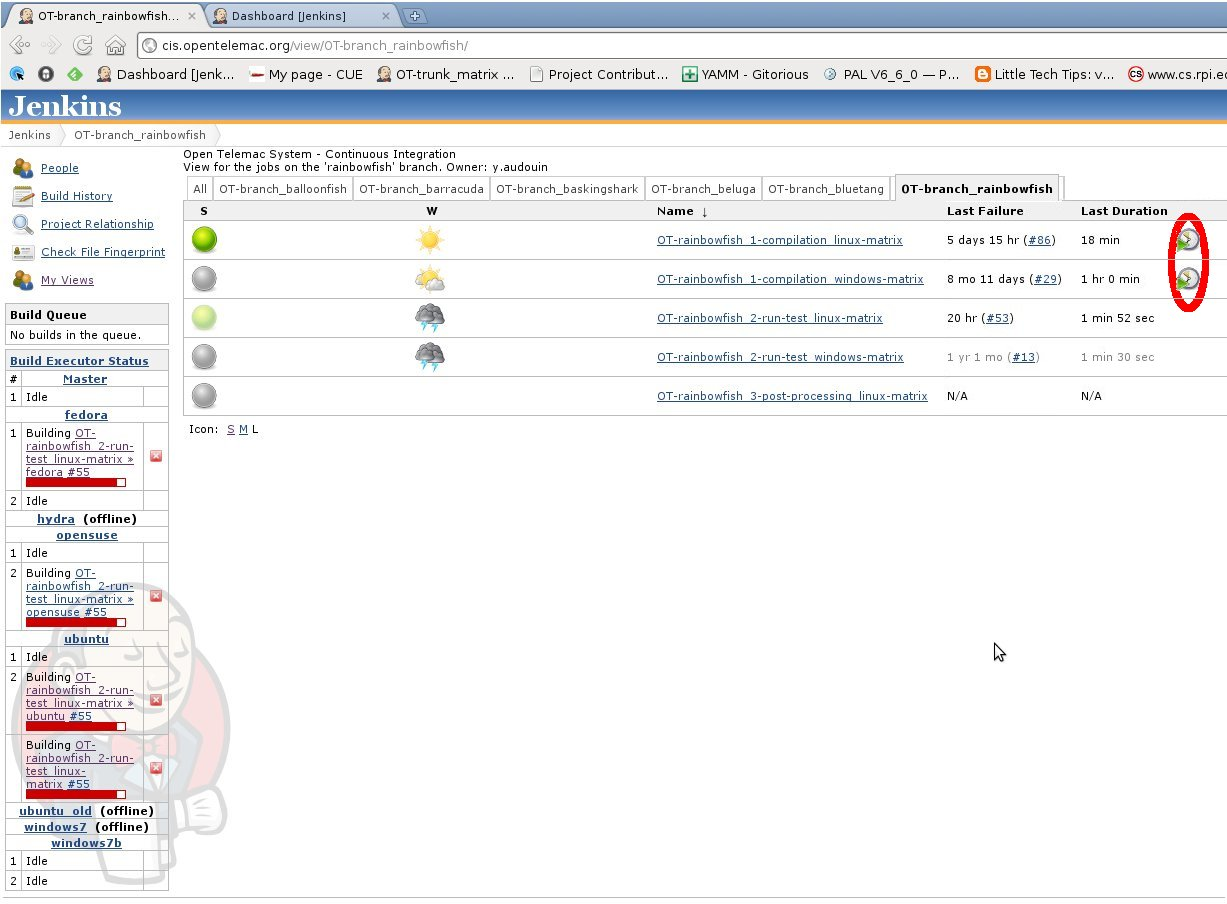
\includegraphics[scale=0.35]{graphics/cis-main.jpg}
    \caption{CIS Branch Page}
    \label{fig:cis-main}
\end{figure}
%
Click on the button in the red circle to launch the job. If you do not see that
button check that you are logged in. This will lead you to the page on Fig
\ref{fig:cis-run-job}.
%
\begin{figure}[H]
    \centering
    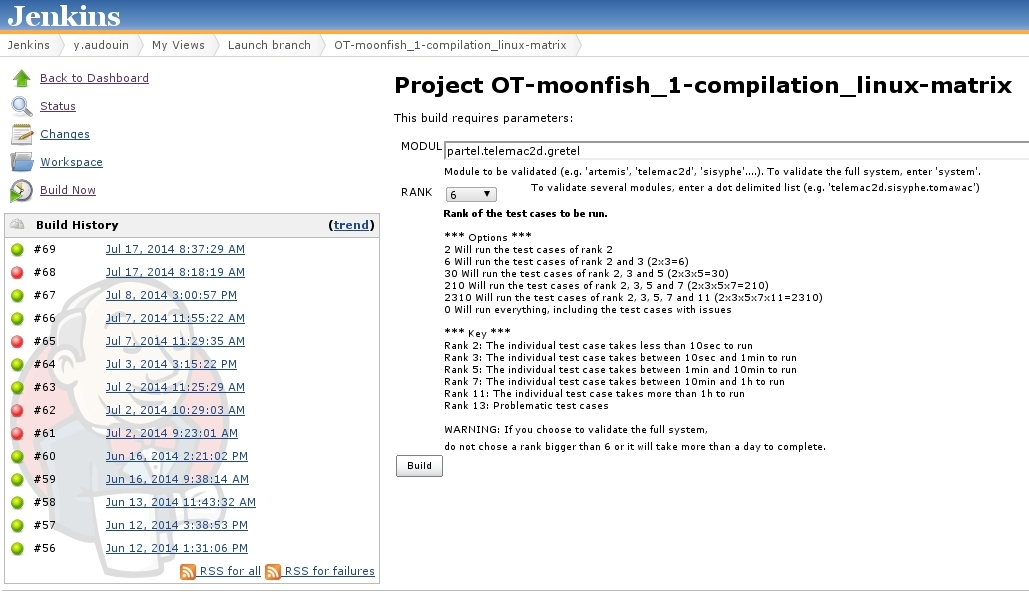
\includegraphics[scale=0.35]{graphics/cis-run-job.jpg}
    \caption{CIS Job execution}
    \label{fig:cis-run-job}
\end{figure}
%
To run the validation on your branch the following information are needed:
\begin{itemize}
\item The modules to run, if you want to run the simulation on only one module
do not forget to add partel and gretel as well to be able to run in parallel,
for exemple "partel.telemac2d.telemac3d.gretel" will run the validation on
telemac2d and telemac3d.

Writing "system" will run the validation on all the modules this is what you
need to validate a development before integration.
\item The level of complexity of test cases to run. The higher the number the
longer the test cases simulation is. For validation of a development 0 is
needed.
\end{itemize} 

If you wanna run the validation locally you need to type one the following commands:
\begin{lstlisting}[language=bash]
validateTELEMAC.py -m module
validateTELEMAC.py --ncsize=3
validateTELEMAC.py
\end{lstlisting}
The first one will launch the validate on a specify list of modules (for example
"telemac2d", "tomawac artemis").
The second one will launch the validation on the whole system but for the
parallel test cases it will replace the number of processors by 3.
The third one will run the validation on the whole system
%
%
\section{Get the listing of the test}
%
%
To see the output of the job you need to follow the step described in Fig
\ref{fig:cis-to-listing}. For step 2 you need to click on the Linux
distribution you want want to get the listing from.  For information only the
ubuntu configuration runs the test cases in parallel.
%
\begin{figure}[H]
    \centering
    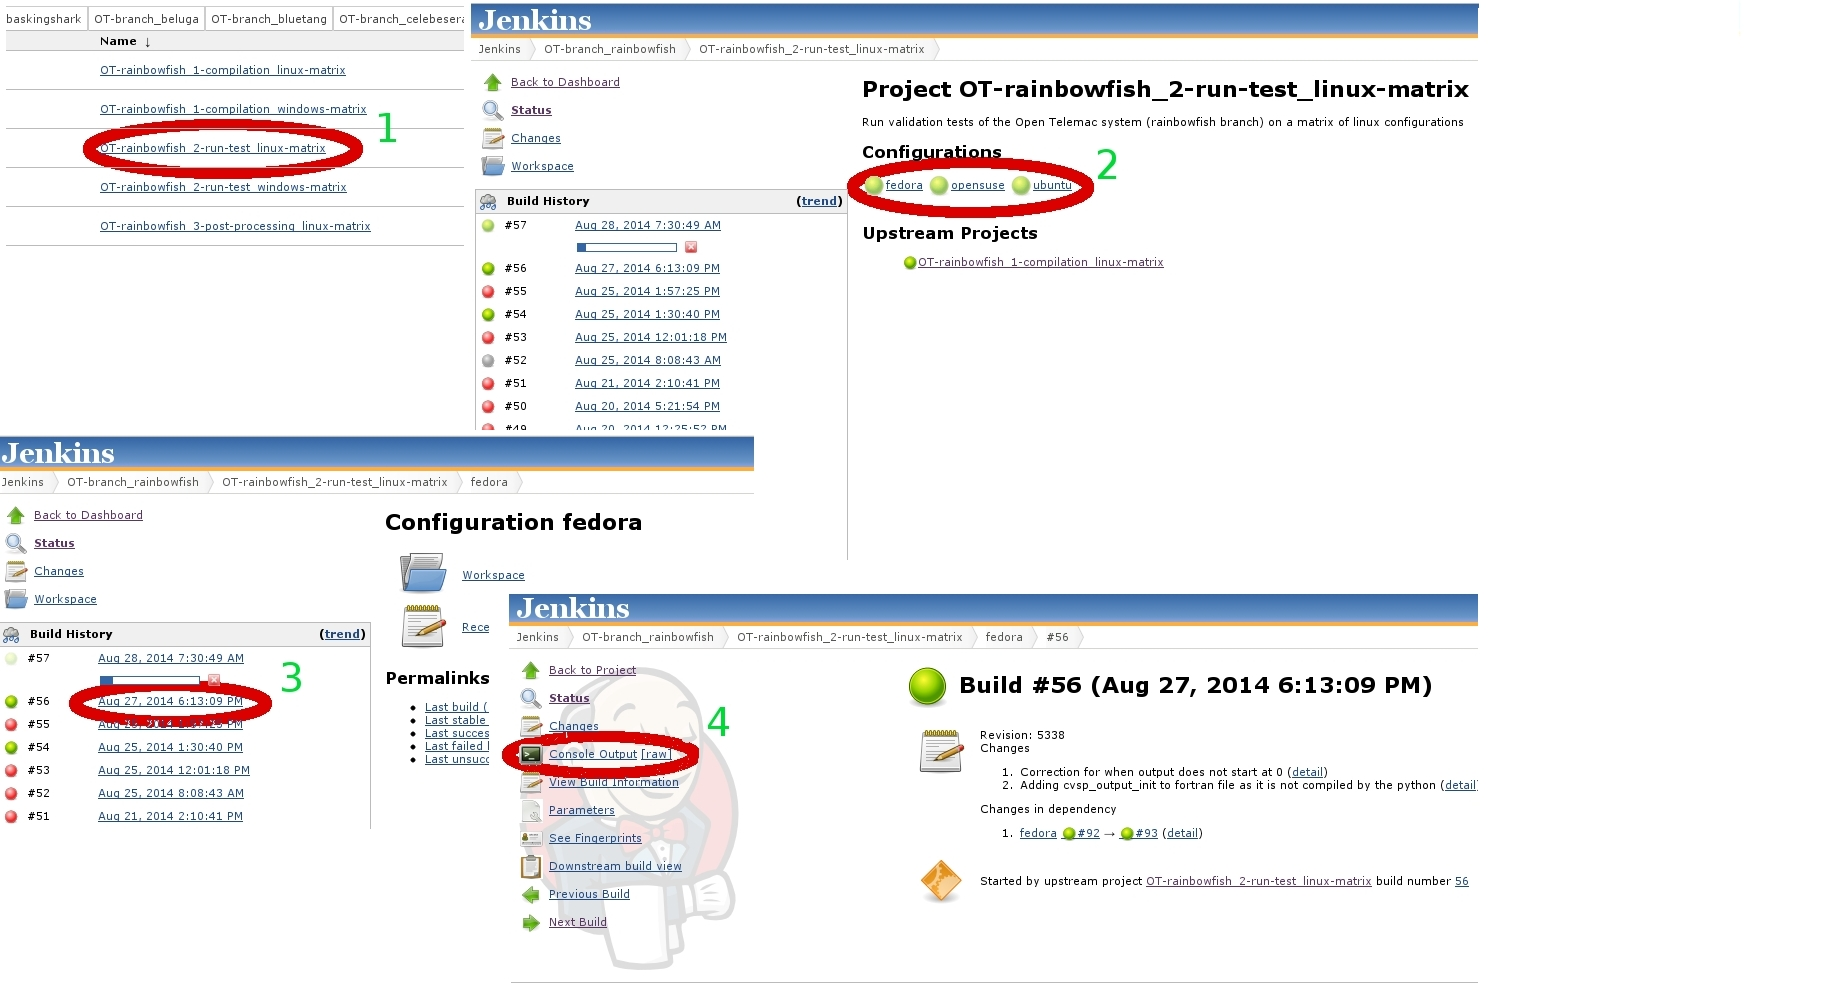
\includegraphics[scale=0.3]{graphics/cis-to-listing.jpg}
    \caption{Process to get the listing of a job execution}
    \label{fig:cis-to-listing}
\end{figure}
%
On step 4, clicking on the "raw" button will give you the complete listing as
the "Console Output" button will only give you the tail of the output that you
can see on Fig \ref{fig:cis-listing}.
%
\begin{figure}[H]
    \centering
    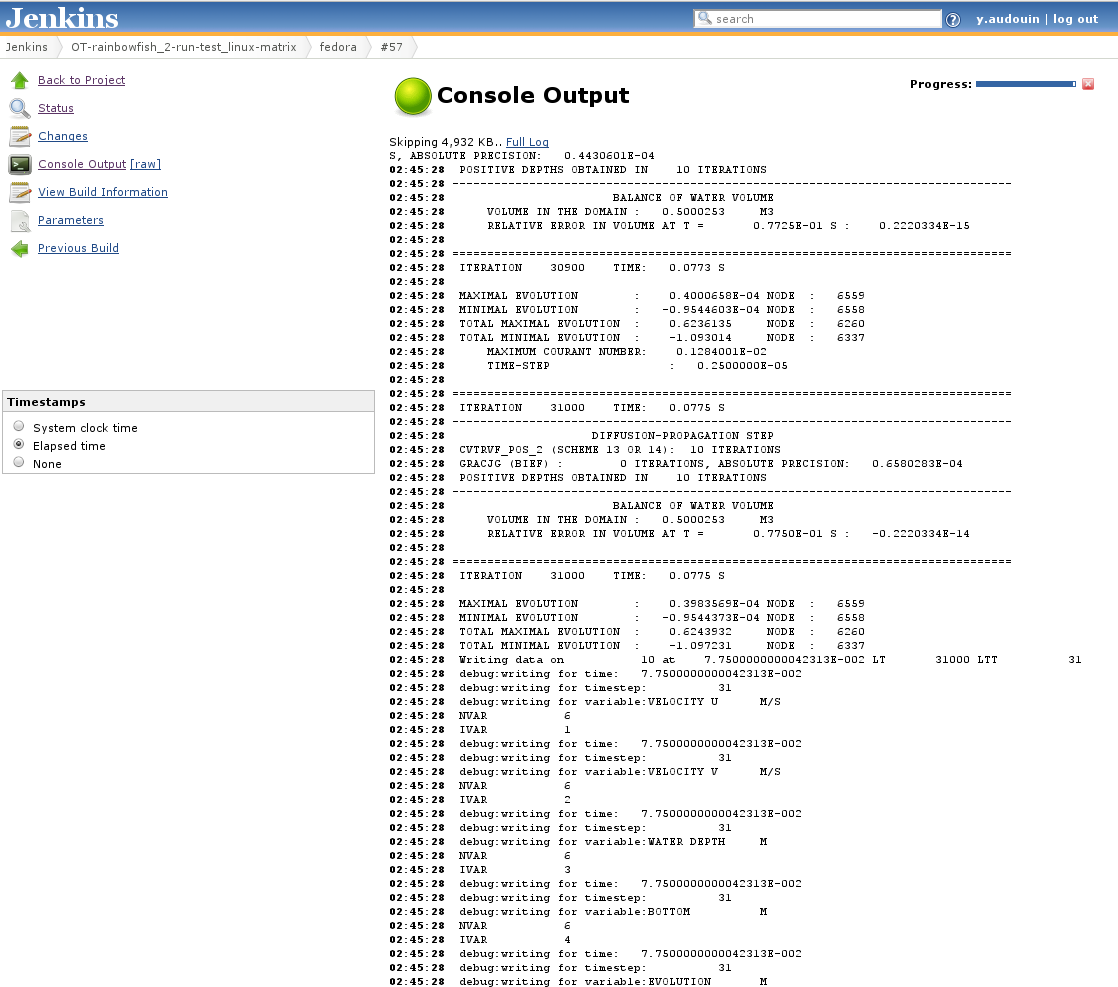
\includegraphics[scale=0.35]{graphics/cis-listing.png}
    \caption{Listing of a job execution}
    \label{fig:cis-listing}
\end{figure}
%

%
%----------------------------------------------------------------------------------------
%     Miscallenous
%----------------------------------------------------------------------------------------
%
%%%%%%%%%%%%%%%%%%%%%%%%%%%%%%%%%%%%%%%%%%%%%%%%%%%%%%%%%%%%%%%%%%%%%%%%
\chapter{Usefull stuff}
%%%%%%%%%%%%%%%%%%%%%%%%%%%%%%%%%%%%%%%%%%%%%%%%%%%%%%%%%%%%%%%%%%%%%%%%
%
\section{Little script to check part of the coding convention}
%
In the trunk version or after (V7.0) you can find a script called
\verb!check_code.sh! that will scan your source code and check for a few points
of the coding convention. You should run this script before submitting your
development. Below is the description the script will give you if you launch it
with the \verb!-h! option. This script is located under the \verb!scripts!
folder in the \telemacsystem directory.
\begin{lstlisting}
Usage: check_code.sh source_path
Script checking some points of the coding convention
for all the .f and .F in the folder given in parameter
It will generate 4 files:
-- indent.log : contains the line where the indentation is
                not a 6 + x*2
-- comments.log : checks that the character used for comments
                  is '!'
-- continuation.log : checks that the character for
                      continuation is '&'
-- lowercase.log : checks that there are no lowercase code
\end{lstlisting}

\section{Adding a new test case}
%
This section will guide you through the hard but needed action of adding a new
case do not frighten it is not that hard. First of all you need to create a new
folder in the examples in the folder corresponding to the module the test case
is for. That folder must contain the following elements:
\begin{itemize}
\item All the \textbf{input} files you need to run the case, and just the input
the files generated by a successful run should not be in the SVN repository.
See the table \ref{tab:namingconv} below for the convention for the naming of
the files.
\item A reference file and/or data to do the validation.
\item The \verb!doc! folder which contains the documentation for the test case
in LaTeX format (See other test cases for example).
\item The xml file to run the test case (See other test cases for example).
\end{itemize}
All the Serafin file must have the extension "slf", the steering case the
extension "cas".

\begin{table}[H]
\begin{center}
%
\caption{Table with contents ranging over several cells horizontally and vertically.}%
\label{tab:namingconv}
%
\begin{tabular*}{0.9\textwidth}{@{\extracolsep{\fill}}cccccc}
\toprule
\toprule
            & geometry, boundary & reference & results & restart & steering and others \\
\midrule
\telemac{2} & geo & f2d & r2d & i2d & t2d \\
\telemac{3} & geo & f3d & r3d & i3d & t3d \\
\tomawac    & geo & f2d & r2d & ini & tom \\
\stbtel     & geo & ref & r2d & ini & stb \\
\sisyphe    & geo & fis & rsi & ini & sis \\
\postel     & geo & ref & res & xxx & p3d \\
\waqtel     & geo & ref & raq & ini & waq \\
\artemis    & geo & frt & r2d & ini & art \\
\end{tabular*}
%
\end{center}
\end{table}

%
%----------------------------------------------------------------------------------------
%     The end of the world as we know it
%----------------------------------------------------------------------------------------
%%%%%%%%%%%%%%%%%%%%%%%%%%%%%%%%%%%%%%%%%%%%%%%%%%%%%%%%%%%%%%%%%%%%%%%%
\chapter{Information to give when your development is over}
%%%%%%%%%%%%%%%%%%%%%%%%%%%%%%%%%%%%%%%%%%%%%%%%%%%%%%%%%%%%%%%%%%%%%%%%
This section will give a list of all the information you need to give to the
person in charge of the integration of your development.
%
\begin{itemize}
\item CUE ticket number.
\item Name of the branch the work is done on.
\item Revision range of work I.e. The revision number of when you started your
  development and when it ended on your SVN branch.
\item A list of the file impacted by the development (See \ref{diff} on how to
create that list).
\item The name of the test cases validating the development (\ref{testcase} on
  how to add a new test case).
\end{itemize}

All those information should be written in the CUE ticket as well.


\end{document}
